\documentclass[twoside]{book}

% Packages required by doxygen
\usepackage{calc}
\usepackage{doxygen}
\usepackage{graphicx}
\usepackage[utf8]{inputenc}
\usepackage{makeidx}
\usepackage{multicol}
\usepackage{multirow}
\usepackage{textcomp}
\usepackage[table]{xcolor}

% Font selection
\usepackage[T1]{fontenc}
\usepackage{mathptmx}
\usepackage[scaled=.90]{helvet}
\usepackage{courier}
\usepackage{amssymb}
\usepackage{sectsty}
\renewcommand{\familydefault}{\sfdefault}
\allsectionsfont{%
  \fontseries{bc}\selectfont%
  \color{darkgray}%
}
\renewcommand{\DoxyLabelFont}{%
  \fontseries{bc}\selectfont%
  \color{darkgray}%
}

% Page & text layout
\usepackage{geometry}
\geometry{%
  a4paper,%
  top=2.5cm,%
  bottom=2.5cm,%
  left=2.5cm,%
  right=2.5cm%
}
\tolerance=750
\hfuzz=15pt
\hbadness=750
\setlength{\emergencystretch}{15pt}
\setlength{\parindent}{0cm}
\setlength{\parskip}{0.2cm}
\makeatletter
\renewcommand{\paragraph}{%
  \@startsection{paragraph}{4}{0ex}{-1.0ex}{1.0ex}{%
    \normalfont\normalsize\bfseries\SS@parafont%
  }%
}
\renewcommand{\subparagraph}{%
  \@startsection{subparagraph}{5}{0ex}{-1.0ex}{1.0ex}{%
    \normalfont\normalsize\bfseries\SS@subparafont%
  }%
}
\makeatother

% Headers & footers
\usepackage{fancyhdr}
\pagestyle{fancyplain}
\fancyhead[LE]{\fancyplain{}{\bfseries\thepage}}
\fancyhead[CE]{\fancyplain{}{}}
\fancyhead[RE]{\fancyplain{}{\bfseries\leftmark}}
\fancyhead[LO]{\fancyplain{}{\bfseries\rightmark}}
\fancyhead[CO]{\fancyplain{}{}}
\fancyhead[RO]{\fancyplain{}{\bfseries\thepage}}
\fancyfoot[LE]{\fancyplain{}{}}
\fancyfoot[CE]{\fancyplain{}{}}
\fancyfoot[RE]{\fancyplain{}{\bfseries\scriptsize Generated on Sun Sep 29 2013 22\-:08\-:52 for Prosco\-F\-X by Doxygen }}
\fancyfoot[LO]{\fancyplain{}{\bfseries\scriptsize Generated on Sun Sep 29 2013 22\-:08\-:52 for Prosco\-F\-X by Doxygen }}
\fancyfoot[CO]{\fancyplain{}{}}
\fancyfoot[RO]{\fancyplain{}{}}
\renewcommand{\footrulewidth}{0.4pt}
\renewcommand{\chaptermark}[1]{%
  \markboth{#1}{}%
}
\renewcommand{\sectionmark}[1]{%
  \markright{\thesection\ #1}%
}

% Indices & bibliography
\usepackage{natbib}
\usepackage[titles]{tocloft}
\setcounter{tocdepth}{3}
\setcounter{secnumdepth}{5}
\makeindex

% Hyperlinks (required, but should be loaded last)
\usepackage{ifpdf}
\ifpdf
  \usepackage[pdftex,pagebackref=true]{hyperref}
\else
  \usepackage[ps2pdf,pagebackref=true]{hyperref}
\fi
\hypersetup{%
  colorlinks=true,%
  linkcolor=blue,%
  citecolor=blue,%
  unicode%
}

% Custom commands
\newcommand{\clearemptydoublepage}{%
  \newpage{\pagestyle{empty}\cleardoublepage}%
}


%===== C O N T E N T S =====

\begin{document}

% Titlepage & ToC
\hypersetup{pageanchor=false}
\pagenumbering{roman}
\begin{titlepage}
\vspace*{7cm}
\begin{center}%
{\Large Prosco\-F\-X }\\
\vspace*{1cm}
{\large Generated by Doxygen 1.8.5}\\
\vspace*{0.5cm}
{\small Sun Sep 29 2013 22:08:52}\\
\end{center}
\end{titlepage}
\clearemptydoublepage
\tableofcontents
\clearemptydoublepage
\pagenumbering{arabic}
\hypersetup{pageanchor=true}

%--- Begin generated contents ---
\chapter{Namespace Index}
\section{Packages}
Here are the packages with brief descriptions (if available)\-:\begin{DoxyCompactList}
\item\contentsline{section}{\hyperlink{namespace_prosco}{Prosco} }{\pageref{namespace_prosco}}{}
\item\contentsline{section}{\hyperlink{namespace_prosco_1_1_app}{Prosco.\-App} }{\pageref{namespace_prosco_1_1_app}}{}
\item\contentsline{section}{\hyperlink{namespace_prosco_1_1_class}{Prosco.\-Class} }{\pageref{namespace_prosco_1_1_class}}{}
\item\contentsline{section}{\hyperlink{namespace_prosco_1_1_controller}{Prosco.\-Controller} }{\pageref{namespace_prosco_1_1_controller}}{}
\end{DoxyCompactList}

\chapter{Hierarchical Index}
\section{Class Hierarchy}
This inheritance list is sorted roughly, but not completely, alphabetically\-:\begin{DoxyCompactList}
\item \contentsline{section}{Prosco.\-Class.\-Class\-B\-D\-Classes}{\pageref{class_prosco_1_1_class_1_1_class_b_d_classes}}{}
\item \contentsline{section}{Prosco.\-Class.\-Class\-B\-D\-Ecole}{\pageref{class_prosco_1_1_class_1_1_class_b_d_ecole}}{}
\item \contentsline{section}{Prosco.\-Class.\-Connect\-B\-D}{\pageref{class_prosco_1_1_class_1_1_connect_b_d}}{}
\item Anchor\-Pane\begin{DoxyCompactList}
\item \contentsline{section}{Prosco.\-Class.\-Inner\-Fxml\-Control}{\pageref{class_prosco_1_1_class_1_1_inner_fxml_control}}{}
\item \contentsline{section}{Prosco.\-Controller.\-Event\-Controller\-Start\-View}{\pageref{class_prosco_1_1_controller_1_1_event_controller_start_view}}{}
\item \contentsline{section}{Prosco.\-Controller.\-Event\-Controller\-View\-Info\-Ecole}{\pageref{class_prosco_1_1_controller_1_1_event_controller_view_info_ecole}}{}
\end{DoxyCompactList}
\item Application\begin{DoxyCompactList}
\item \contentsline{section}{Prosco.\-App.\-App}{\pageref{class_prosco_1_1_app_1_1_app}}{}
\end{DoxyCompactList}
\item Initializable\begin{DoxyCompactList}
\item \contentsline{section}{Prosco.\-Controller.\-Event\-Controller\-Start\-View}{\pageref{class_prosco_1_1_controller_1_1_event_controller_start_view}}{}
\item \contentsline{section}{Prosco.\-Controller.\-Event\-Controller\-View\-Info\-Ecole}{\pageref{class_prosco_1_1_controller_1_1_event_controller_view_info_ecole}}{}
\end{DoxyCompactList}
\end{DoxyCompactList}

\chapter{Class Index}
\section{Class List}
Here are the classes, structs, unions and interfaces with brief descriptions\-:\begin{DoxyCompactList}
\item\contentsline{section}{\hyperlink{class_prosco_1_1_app_1_1_app}{Prosco.\-App.\-App} }{\pageref{class_prosco_1_1_app_1_1_app}}{}
\item\contentsline{section}{\hyperlink{class_prosco_1_1_class_1_1_class_b_d_classes}{Prosco.\-Class.\-Class\-B\-D\-Classes} }{\pageref{class_prosco_1_1_class_1_1_class_b_d_classes}}{}
\item\contentsline{section}{\hyperlink{class_prosco_1_1_class_1_1_class_b_d_ecole}{Prosco.\-Class.\-Class\-B\-D\-Ecole} }{\pageref{class_prosco_1_1_class_1_1_class_b_d_ecole}}{}
\item\contentsline{section}{\hyperlink{class_prosco_1_1_class_1_1_connect_b_d}{Prosco.\-Class.\-Connect\-B\-D} }{\pageref{class_prosco_1_1_class_1_1_connect_b_d}}{}
\item\contentsline{section}{\hyperlink{class_prosco_1_1_controller_1_1_event_controller_start_view}{Prosco.\-Controller.\-Event\-Controller\-Start\-View} }{\pageref{class_prosco_1_1_controller_1_1_event_controller_start_view}}{}
\item\contentsline{section}{\hyperlink{class_prosco_1_1_controller_1_1_event_controller_view_info_ecole}{Prosco.\-Controller.\-Event\-Controller\-View\-Info\-Ecole} }{\pageref{class_prosco_1_1_controller_1_1_event_controller_view_info_ecole}}{}
\item\contentsline{section}{\hyperlink{class_prosco_1_1_class_1_1_inner_fxml_control}{Prosco.\-Class.\-Inner\-Fxml\-Control} }{\pageref{class_prosco_1_1_class_1_1_inner_fxml_control}}{}
\end{DoxyCompactList}

\chapter{File Index}
\section{File List}
Here is a list of all files with brief descriptions\-:\begin{DoxyCompactList}
\item\contentsline{section}{src/\-Prosco/\-App/\hyperlink{_app_8java}{App.\-java} }{\pageref{_app_8java}}{}
\item\contentsline{section}{src/\-Prosco/\-Class/\hyperlink{_class_b_d_classes_8java}{Class\-B\-D\-Classes.\-java} }{\pageref{_class_b_d_classes_8java}}{}
\item\contentsline{section}{src/\-Prosco/\-Class/\hyperlink{_class_b_d_ecole_8java}{Class\-B\-D\-Ecole.\-java} }{\pageref{_class_b_d_ecole_8java}}{}
\item\contentsline{section}{src/\-Prosco/\-Class/\hyperlink{_connect_b_d_8java}{Connect\-B\-D.\-java} \\*Classe qui permet de cr�er la connexion aux bases de donn�es }{\pageref{_connect_b_d_8java}}{}
\item\contentsline{section}{src/\-Prosco/\-Class/\hyperlink{_inner_fxml_control_8java}{Inner\-Fxml\-Control.\-java} }{\pageref{_inner_fxml_control_8java}}{}
\item\contentsline{section}{src/\-Prosco/\-Controller/\hyperlink{_event_controller_start_view_8java}{Event\-Controller\-Start\-View.\-java} }{\pageref{_event_controller_start_view_8java}}{}
\item\contentsline{section}{src/\-Prosco/\-Controller/\hyperlink{_event_controller_view_info_ecole_8java}{Event\-Controller\-View\-Info\-Ecole.\-java} }{\pageref{_event_controller_view_info_ecole_8java}}{}
\end{DoxyCompactList}

\chapter{Namespace Documentation}
\hypertarget{namespace_prosco}{\section{Package Prosco}
\label{namespace_prosco}\index{Prosco@{Prosco}}
}
\subsection*{Packages}
\begin{DoxyCompactItemize}
\item 
package \hyperlink{namespace_prosco_1_1_app}{App}
\item 
package \hyperlink{namespace_prosco_1_1_class}{Class}
\item 
package \hyperlink{namespace_prosco_1_1_controller}{Controller}
\end{DoxyCompactItemize}

\hypertarget{namespace_prosco_1_1_app}{\section{Package Prosco.\-App}
\label{namespace_prosco_1_1_app}\index{Prosco.\-App@{Prosco.\-App}}
}
\subsection*{Classes}
\begin{DoxyCompactItemize}
\item 
class \hyperlink{class_prosco_1_1_app_1_1_app}{App}
\end{DoxyCompactItemize}

\hypertarget{namespace_prosco_1_1_class}{\section{Package Prosco.\-Class}
\label{namespace_prosco_1_1_class}\index{Prosco.\-Class@{Prosco.\-Class}}
}
\subsection*{Classes}
\begin{DoxyCompactItemize}
\item 
class \hyperlink{class_prosco_1_1_class_1_1_class_b_d_classes}{Class\-B\-D\-Classes}
\item 
class \hyperlink{class_prosco_1_1_class_1_1_class_b_d_ecole}{Class\-B\-D\-Ecole}
\item 
class \hyperlink{class_prosco_1_1_class_1_1_connect_b_d}{Connect\-B\-D}
\item 
class \hyperlink{class_prosco_1_1_class_1_1_inner_fxml_control}{Inner\-Fxml\-Control}
\end{DoxyCompactItemize}

\hypertarget{namespace_prosco_1_1_controller}{\section{Package Prosco.\-Controller}
\label{namespace_prosco_1_1_controller}\index{Prosco.\-Controller@{Prosco.\-Controller}}
}
\subsection*{Classes}
\begin{DoxyCompactItemize}
\item 
class \hyperlink{class_prosco_1_1_controller_1_1_event_controller_start_view}{Event\-Controller\-Start\-View}
\item 
class \hyperlink{class_prosco_1_1_controller_1_1_event_controller_view_info_ecole}{Event\-Controller\-View\-Info\-Ecole}
\end{DoxyCompactItemize}

\chapter{Class Documentation}
\hypertarget{class_prosco_1_1_app_1_1_app}{\section{Prosco.\-App.\-App Class Reference}
\label{class_prosco_1_1_app_1_1_app}\index{Prosco.\-App.\-App@{Prosco.\-App.\-App}}
}
Inheritance diagram for Prosco.\-App.\-App\-:\begin{figure}[H]
\begin{center}
\leavevmode
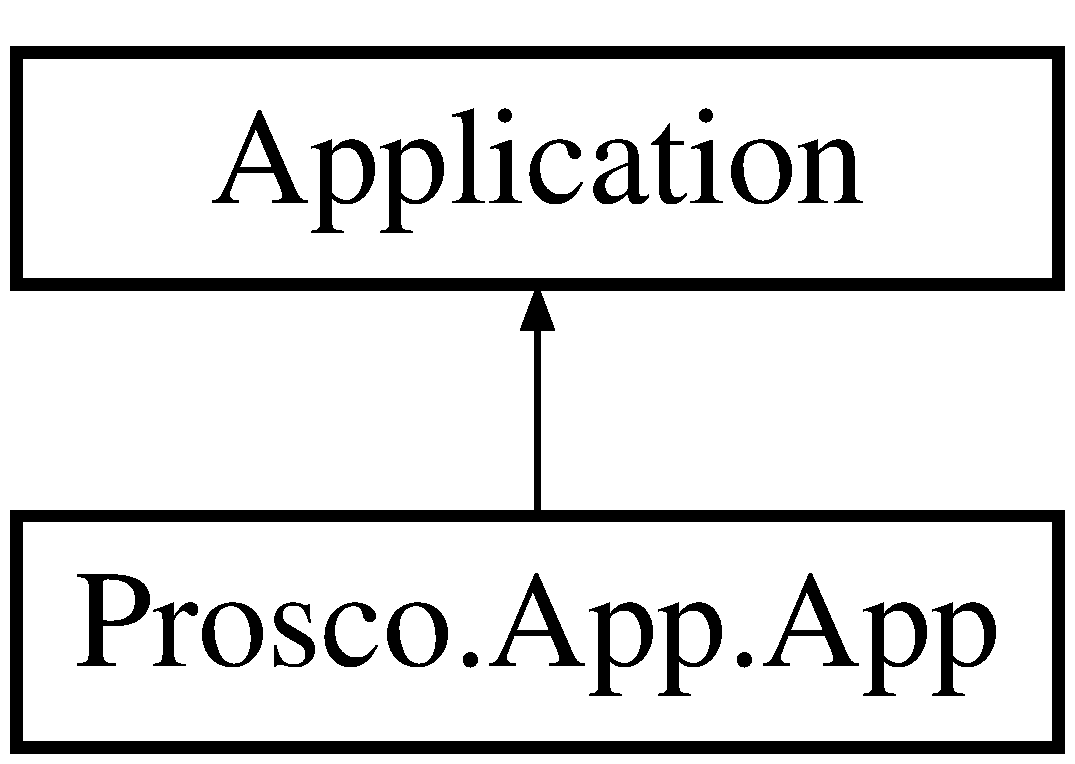
\includegraphics[height=2.000000cm]{class_prosco_1_1_app_1_1_app}
\end{center}
\end{figure}
\subsection*{Public Member Functions}
\begin{DoxyCompactItemize}
\item 
void \hyperlink{class_prosco_1_1_app_1_1_app_ac7a278030dcc09c4555a02a486053337}{start} (Stage primary\-Stage)  throws I\-O\-Exception 
\end{DoxyCompactItemize}
\subsection*{Static Public Member Functions}
\begin{DoxyCompactItemize}
\item 
static Object\-Property$<$ Stage $>$ \hyperlink{class_prosco_1_1_app_1_1_app_ad017ef8c92c342dcf88a78e3d1a9be96}{current\-Stage\-Property} ()
\item 
static Stage \hyperlink{class_prosco_1_1_app_1_1_app_a5acb7d1f45c619f4ff59c966d02fa23c}{get\-Current\-Stage} ()
\item 
static void \hyperlink{class_prosco_1_1_app_1_1_app_aa3c0f99606025770f5de6cc5a1e4f5c9}{main} (String\mbox{[}$\,$\mbox{]} args)
\end{DoxyCompactItemize}
\subsection*{Static Private Attributes}
\begin{DoxyCompactItemize}
\item 
static Object\-Property$<$ Stage $>$ \hyperlink{class_prosco_1_1_app_1_1_app_a625c10eb01309fae38fdcc9cfcb1bb73}{current\-Stage}
\end{DoxyCompactItemize}


\subsection{Member Function Documentation}
\hypertarget{class_prosco_1_1_app_1_1_app_ad017ef8c92c342dcf88a78e3d1a9be96}{\index{Prosco\-::\-App\-::\-App@{Prosco\-::\-App\-::\-App}!current\-Stage\-Property@{current\-Stage\-Property}}
\index{current\-Stage\-Property@{current\-Stage\-Property}!Prosco::App::App@{Prosco\-::\-App\-::\-App}}
\subsubsection[{current\-Stage\-Property}]{\setlength{\rightskip}{0pt plus 5cm}static Object\-Property$<$Stage$>$ Prosco.\-App.\-App.\-current\-Stage\-Property (
\begin{DoxyParamCaption}
{}
\end{DoxyParamCaption}
)\hspace{0.3cm}{\ttfamily [static]}}}\label{class_prosco_1_1_app_1_1_app_ad017ef8c92c342dcf88a78e3d1a9be96}
\hypertarget{class_prosco_1_1_app_1_1_app_a5acb7d1f45c619f4ff59c966d02fa23c}{\index{Prosco\-::\-App\-::\-App@{Prosco\-::\-App\-::\-App}!get\-Current\-Stage@{get\-Current\-Stage}}
\index{get\-Current\-Stage@{get\-Current\-Stage}!Prosco::App::App@{Prosco\-::\-App\-::\-App}}
\subsubsection[{get\-Current\-Stage}]{\setlength{\rightskip}{0pt plus 5cm}static Stage Prosco.\-App.\-App.\-get\-Current\-Stage (
\begin{DoxyParamCaption}
{}
\end{DoxyParamCaption}
)\hspace{0.3cm}{\ttfamily [static]}}}\label{class_prosco_1_1_app_1_1_app_a5acb7d1f45c619f4ff59c966d02fa23c}
\hypertarget{class_prosco_1_1_app_1_1_app_aa3c0f99606025770f5de6cc5a1e4f5c9}{\index{Prosco\-::\-App\-::\-App@{Prosco\-::\-App\-::\-App}!main@{main}}
\index{main@{main}!Prosco::App::App@{Prosco\-::\-App\-::\-App}}
\subsubsection[{main}]{\setlength{\rightskip}{0pt plus 5cm}static void Prosco.\-App.\-App.\-main (
\begin{DoxyParamCaption}
\item[{String\mbox{[}$\,$\mbox{]}}]{args}
\end{DoxyParamCaption}
)\hspace{0.3cm}{\ttfamily [static]}}}\label{class_prosco_1_1_app_1_1_app_aa3c0f99606025770f5de6cc5a1e4f5c9}
\hypertarget{class_prosco_1_1_app_1_1_app_ac7a278030dcc09c4555a02a486053337}{\index{Prosco\-::\-App\-::\-App@{Prosco\-::\-App\-::\-App}!start@{start}}
\index{start@{start}!Prosco::App::App@{Prosco\-::\-App\-::\-App}}
\subsubsection[{start}]{\setlength{\rightskip}{0pt plus 5cm}void Prosco.\-App.\-App.\-start (
\begin{DoxyParamCaption}
\item[{Stage}]{primary\-Stage}
\end{DoxyParamCaption}
) throws I\-O\-Exception}}\label{class_prosco_1_1_app_1_1_app_ac7a278030dcc09c4555a02a486053337}


\subsection{Member Data Documentation}
\hypertarget{class_prosco_1_1_app_1_1_app_a625c10eb01309fae38fdcc9cfcb1bb73}{\index{Prosco\-::\-App\-::\-App@{Prosco\-::\-App\-::\-App}!current\-Stage@{current\-Stage}}
\index{current\-Stage@{current\-Stage}!Prosco::App::App@{Prosco\-::\-App\-::\-App}}
\subsubsection[{current\-Stage}]{\setlength{\rightskip}{0pt plus 5cm}Object\-Property$<$Stage$>$ Prosco.\-App.\-App.\-current\-Stage\hspace{0.3cm}{\ttfamily [static]}, {\ttfamily [private]}}}\label{class_prosco_1_1_app_1_1_app_a625c10eb01309fae38fdcc9cfcb1bb73}


The documentation for this class was generated from the following file\-:\begin{DoxyCompactItemize}
\item 
src/\-Prosco/\-App/\hyperlink{_app_8java}{App.\-java}\end{DoxyCompactItemize}

\hypertarget{class_prosco_1_1_class_1_1_class_b_d_classes}{\section{Prosco.\-Class.\-Class\-B\-D\-Classes Class Reference}
\label{class_prosco_1_1_class_1_1_class_b_d_classes}\index{Prosco.\-Class.\-Class\-B\-D\-Classes@{Prosco.\-Class.\-Class\-B\-D\-Classes}}
}
\subsection*{Public Member Functions}
\begin{DoxyCompactItemize}
\item 
\hyperlink{class_prosco_1_1_class_1_1_class_b_d_classes_a067c2a6918ef23ae11895d8610c16dcf}{Class\-B\-D\-Classes} (int E\-C\-O\-L\-E\-S\-\_\-id\-Ecole)
\end{DoxyCompactItemize}


\subsection{Constructor \& Destructor Documentation}
\hypertarget{class_prosco_1_1_class_1_1_class_b_d_classes_a067c2a6918ef23ae11895d8610c16dcf}{\index{Prosco\-::\-Class\-::\-Class\-B\-D\-Classes@{Prosco\-::\-Class\-::\-Class\-B\-D\-Classes}!Class\-B\-D\-Classes@{Class\-B\-D\-Classes}}
\index{Class\-B\-D\-Classes@{Class\-B\-D\-Classes}!Prosco::Class::ClassBDClasses@{Prosco\-::\-Class\-::\-Class\-B\-D\-Classes}}
\subsubsection[{Class\-B\-D\-Classes}]{\setlength{\rightskip}{0pt plus 5cm}Prosco.\-Class.\-Class\-B\-D\-Classes.\-Class\-B\-D\-Classes (
\begin{DoxyParamCaption}
\item[{int}]{E\-C\-O\-L\-E\-S\-\_\-id\-Ecole}
\end{DoxyParamCaption}
)}}\label{class_prosco_1_1_class_1_1_class_b_d_classes_a067c2a6918ef23ae11895d8610c16dcf}


The documentation for this class was generated from the following file\-:\begin{DoxyCompactItemize}
\item 
src/\-Prosco/\-Class/\hyperlink{_class_b_d_classes_8java}{Class\-B\-D\-Classes.\-java}\end{DoxyCompactItemize}

\hypertarget{class_prosco_1_1_class_1_1_class_b_d_ecole}{\section{Prosco.\-Class.\-Class\-B\-D\-Ecole Class Reference}
\label{class_prosco_1_1_class_1_1_class_b_d_ecole}\index{Prosco.\-Class.\-Class\-B\-D\-Ecole@{Prosco.\-Class.\-Class\-B\-D\-Ecole}}
}
\subsection*{Public Member Functions}
\begin{DoxyCompactItemize}
\item 
\hyperlink{class_prosco_1_1_class_1_1_class_b_d_ecole_a5b607d51eb6d2fbc49e653f7be26d52f}{Class\-B\-D\-Ecole} (String N\-O\-M\-E\-C\-O\-L\-E)
\item 
String \hyperlink{class_prosco_1_1_class_1_1_class_b_d_ecole_aa1aa568ceeda8e6be965918f2f4ee326}{get\-Nom\-Ecole} ()
\item 
void \hyperlink{class_prosco_1_1_class_1_1_class_b_d_ecole_ac6bcca29b5dd3986ec40a4dbc615e2aa}{set\-Nom\-Ecole} (String new\-Nom\-Ecole)
\item 
int \hyperlink{class_prosco_1_1_class_1_1_class_b_d_ecole_a954f35bb6410dcac712cd71949858126}{get\-Id\-Ecole} ()
\item 
String \hyperlink{class_prosco_1_1_class_1_1_class_b_d_ecole_a208dd2174b21706cfcf8528089104b4c}{get\-Adresse1} ()
\item 
void \hyperlink{class_prosco_1_1_class_1_1_class_b_d_ecole_aa9f06c5c6ec93899825335cde0323099}{set\-Adresse1} (String new\-Adresse)
\item 
String \hyperlink{class_prosco_1_1_class_1_1_class_b_d_ecole_a8c91466e414ebca4f0603666a13bb189}{get\-Adresse2} ()
\item 
void \hyperlink{class_prosco_1_1_class_1_1_class_b_d_ecole_a86ae4c82f7c9eb9185d43b0144b84786}{set\-Adresse2} (String new\-Adresse)
\item 
int \hyperlink{class_prosco_1_1_class_1_1_class_b_d_ecole_ac1e324b6078a984c6fe019c18da47393}{get\-Code\-Postal} ()
\item 
void \hyperlink{class_prosco_1_1_class_1_1_class_b_d_ecole_aa5d09349160fdea46fe2df83ff0d129e}{set\-Code\-Postal} (int new\-Code\-Postal)
\item 
String \hyperlink{class_prosco_1_1_class_1_1_class_b_d_ecole_ad58a6aaa25efcbc7a18149b20b53ea69}{get\-Ville} ()
\item 
void \hyperlink{class_prosco_1_1_class_1_1_class_b_d_ecole_a1d7627287937a72d51ee49c59126da9e}{set\-Ville} (String new\-Ville)
\item 
String \hyperlink{class_prosco_1_1_class_1_1_class_b_d_ecole_a7b933fb03ad723a192032112a9bdc3cf}{get\-Nom\-Directeur} ()
\item 
void \hyperlink{class_prosco_1_1_class_1_1_class_b_d_ecole_abda7dcc90b733a5905f0db57da1cb3c5}{set\-Nom\-Directeur} (String new\-Nom\-Directeur)
\item 
String \hyperlink{class_prosco_1_1_class_1_1_class_b_d_ecole_a6b582d7b1b4835e22bc94a1bf4f9aed9}{get\-Nom\-Responsable} ()
\item 
void \hyperlink{class_prosco_1_1_class_1_1_class_b_d_ecole_aad46b44b724b47941a19371caa0846fa}{set\-Nom\-Responsable} (String new\-Nom\-Responsable)
\item 
void \hyperlink{class_prosco_1_1_class_1_1_class_b_d_ecole_ab6b7b3c0e692c439fda4fcdf280dedac}{charger\-Ecole} (String I\-D\-E\-C\-O\-L\-E, Object object)  throws I\-O\-Exception 
\end{DoxyCompactItemize}


\subsection{Constructor \& Destructor Documentation}
\hypertarget{class_prosco_1_1_class_1_1_class_b_d_ecole_a5b607d51eb6d2fbc49e653f7be26d52f}{\index{Prosco\-::\-Class\-::\-Class\-B\-D\-Ecole@{Prosco\-::\-Class\-::\-Class\-B\-D\-Ecole}!Class\-B\-D\-Ecole@{Class\-B\-D\-Ecole}}
\index{Class\-B\-D\-Ecole@{Class\-B\-D\-Ecole}!Prosco::Class::ClassBDEcole@{Prosco\-::\-Class\-::\-Class\-B\-D\-Ecole}}
\subsubsection[{Class\-B\-D\-Ecole}]{\setlength{\rightskip}{0pt plus 5cm}Prosco.\-Class.\-Class\-B\-D\-Ecole.\-Class\-B\-D\-Ecole (
\begin{DoxyParamCaption}
\item[{String}]{N\-O\-M\-E\-C\-O\-L\-E}
\end{DoxyParamCaption}
)}}\label{class_prosco_1_1_class_1_1_class_b_d_ecole_a5b607d51eb6d2fbc49e653f7be26d52f}


\subsection{Member Function Documentation}
\hypertarget{class_prosco_1_1_class_1_1_class_b_d_ecole_ab6b7b3c0e692c439fda4fcdf280dedac}{\index{Prosco\-::\-Class\-::\-Class\-B\-D\-Ecole@{Prosco\-::\-Class\-::\-Class\-B\-D\-Ecole}!charger\-Ecole@{charger\-Ecole}}
\index{charger\-Ecole@{charger\-Ecole}!Prosco::Class::ClassBDEcole@{Prosco\-::\-Class\-::\-Class\-B\-D\-Ecole}}
\subsubsection[{charger\-Ecole}]{\setlength{\rightskip}{0pt plus 5cm}void Prosco.\-Class.\-Class\-B\-D\-Ecole.\-charger\-Ecole (
\begin{DoxyParamCaption}
\item[{String}]{I\-D\-E\-C\-O\-L\-E, }
\item[{Object}]{object}
\end{DoxyParamCaption}
) throws I\-O\-Exception}}\label{class_prosco_1_1_class_1_1_class_b_d_ecole_ab6b7b3c0e692c439fda4fcdf280dedac}
\hypertarget{class_prosco_1_1_class_1_1_class_b_d_ecole_a208dd2174b21706cfcf8528089104b4c}{\index{Prosco\-::\-Class\-::\-Class\-B\-D\-Ecole@{Prosco\-::\-Class\-::\-Class\-B\-D\-Ecole}!get\-Adresse1@{get\-Adresse1}}
\index{get\-Adresse1@{get\-Adresse1}!Prosco::Class::ClassBDEcole@{Prosco\-::\-Class\-::\-Class\-B\-D\-Ecole}}
\subsubsection[{get\-Adresse1}]{\setlength{\rightskip}{0pt plus 5cm}String Prosco.\-Class.\-Class\-B\-D\-Ecole.\-get\-Adresse1 (
\begin{DoxyParamCaption}
{}
\end{DoxyParamCaption}
)}}\label{class_prosco_1_1_class_1_1_class_b_d_ecole_a208dd2174b21706cfcf8528089104b4c}
\hypertarget{class_prosco_1_1_class_1_1_class_b_d_ecole_a8c91466e414ebca4f0603666a13bb189}{\index{Prosco\-::\-Class\-::\-Class\-B\-D\-Ecole@{Prosco\-::\-Class\-::\-Class\-B\-D\-Ecole}!get\-Adresse2@{get\-Adresse2}}
\index{get\-Adresse2@{get\-Adresse2}!Prosco::Class::ClassBDEcole@{Prosco\-::\-Class\-::\-Class\-B\-D\-Ecole}}
\subsubsection[{get\-Adresse2}]{\setlength{\rightskip}{0pt plus 5cm}String Prosco.\-Class.\-Class\-B\-D\-Ecole.\-get\-Adresse2 (
\begin{DoxyParamCaption}
{}
\end{DoxyParamCaption}
)}}\label{class_prosco_1_1_class_1_1_class_b_d_ecole_a8c91466e414ebca4f0603666a13bb189}
\hypertarget{class_prosco_1_1_class_1_1_class_b_d_ecole_ac1e324b6078a984c6fe019c18da47393}{\index{Prosco\-::\-Class\-::\-Class\-B\-D\-Ecole@{Prosco\-::\-Class\-::\-Class\-B\-D\-Ecole}!get\-Code\-Postal@{get\-Code\-Postal}}
\index{get\-Code\-Postal@{get\-Code\-Postal}!Prosco::Class::ClassBDEcole@{Prosco\-::\-Class\-::\-Class\-B\-D\-Ecole}}
\subsubsection[{get\-Code\-Postal}]{\setlength{\rightskip}{0pt plus 5cm}int Prosco.\-Class.\-Class\-B\-D\-Ecole.\-get\-Code\-Postal (
\begin{DoxyParamCaption}
{}
\end{DoxyParamCaption}
)}}\label{class_prosco_1_1_class_1_1_class_b_d_ecole_ac1e324b6078a984c6fe019c18da47393}
\hypertarget{class_prosco_1_1_class_1_1_class_b_d_ecole_a954f35bb6410dcac712cd71949858126}{\index{Prosco\-::\-Class\-::\-Class\-B\-D\-Ecole@{Prosco\-::\-Class\-::\-Class\-B\-D\-Ecole}!get\-Id\-Ecole@{get\-Id\-Ecole}}
\index{get\-Id\-Ecole@{get\-Id\-Ecole}!Prosco::Class::ClassBDEcole@{Prosco\-::\-Class\-::\-Class\-B\-D\-Ecole}}
\subsubsection[{get\-Id\-Ecole}]{\setlength{\rightskip}{0pt plus 5cm}int Prosco.\-Class.\-Class\-B\-D\-Ecole.\-get\-Id\-Ecole (
\begin{DoxyParamCaption}
{}
\end{DoxyParamCaption}
)}}\label{class_prosco_1_1_class_1_1_class_b_d_ecole_a954f35bb6410dcac712cd71949858126}
\hypertarget{class_prosco_1_1_class_1_1_class_b_d_ecole_a7b933fb03ad723a192032112a9bdc3cf}{\index{Prosco\-::\-Class\-::\-Class\-B\-D\-Ecole@{Prosco\-::\-Class\-::\-Class\-B\-D\-Ecole}!get\-Nom\-Directeur@{get\-Nom\-Directeur}}
\index{get\-Nom\-Directeur@{get\-Nom\-Directeur}!Prosco::Class::ClassBDEcole@{Prosco\-::\-Class\-::\-Class\-B\-D\-Ecole}}
\subsubsection[{get\-Nom\-Directeur}]{\setlength{\rightskip}{0pt plus 5cm}String Prosco.\-Class.\-Class\-B\-D\-Ecole.\-get\-Nom\-Directeur (
\begin{DoxyParamCaption}
{}
\end{DoxyParamCaption}
)}}\label{class_prosco_1_1_class_1_1_class_b_d_ecole_a7b933fb03ad723a192032112a9bdc3cf}
\hypertarget{class_prosco_1_1_class_1_1_class_b_d_ecole_aa1aa568ceeda8e6be965918f2f4ee326}{\index{Prosco\-::\-Class\-::\-Class\-B\-D\-Ecole@{Prosco\-::\-Class\-::\-Class\-B\-D\-Ecole}!get\-Nom\-Ecole@{get\-Nom\-Ecole}}
\index{get\-Nom\-Ecole@{get\-Nom\-Ecole}!Prosco::Class::ClassBDEcole@{Prosco\-::\-Class\-::\-Class\-B\-D\-Ecole}}
\subsubsection[{get\-Nom\-Ecole}]{\setlength{\rightskip}{0pt plus 5cm}String Prosco.\-Class.\-Class\-B\-D\-Ecole.\-get\-Nom\-Ecole (
\begin{DoxyParamCaption}
{}
\end{DoxyParamCaption}
)}}\label{class_prosco_1_1_class_1_1_class_b_d_ecole_aa1aa568ceeda8e6be965918f2f4ee326}
\hypertarget{class_prosco_1_1_class_1_1_class_b_d_ecole_a6b582d7b1b4835e22bc94a1bf4f9aed9}{\index{Prosco\-::\-Class\-::\-Class\-B\-D\-Ecole@{Prosco\-::\-Class\-::\-Class\-B\-D\-Ecole}!get\-Nom\-Responsable@{get\-Nom\-Responsable}}
\index{get\-Nom\-Responsable@{get\-Nom\-Responsable}!Prosco::Class::ClassBDEcole@{Prosco\-::\-Class\-::\-Class\-B\-D\-Ecole}}
\subsubsection[{get\-Nom\-Responsable}]{\setlength{\rightskip}{0pt plus 5cm}String Prosco.\-Class.\-Class\-B\-D\-Ecole.\-get\-Nom\-Responsable (
\begin{DoxyParamCaption}
{}
\end{DoxyParamCaption}
)}}\label{class_prosco_1_1_class_1_1_class_b_d_ecole_a6b582d7b1b4835e22bc94a1bf4f9aed9}
\hypertarget{class_prosco_1_1_class_1_1_class_b_d_ecole_ad58a6aaa25efcbc7a18149b20b53ea69}{\index{Prosco\-::\-Class\-::\-Class\-B\-D\-Ecole@{Prosco\-::\-Class\-::\-Class\-B\-D\-Ecole}!get\-Ville@{get\-Ville}}
\index{get\-Ville@{get\-Ville}!Prosco::Class::ClassBDEcole@{Prosco\-::\-Class\-::\-Class\-B\-D\-Ecole}}
\subsubsection[{get\-Ville}]{\setlength{\rightskip}{0pt plus 5cm}String Prosco.\-Class.\-Class\-B\-D\-Ecole.\-get\-Ville (
\begin{DoxyParamCaption}
{}
\end{DoxyParamCaption}
)}}\label{class_prosco_1_1_class_1_1_class_b_d_ecole_ad58a6aaa25efcbc7a18149b20b53ea69}
\hypertarget{class_prosco_1_1_class_1_1_class_b_d_ecole_aa9f06c5c6ec93899825335cde0323099}{\index{Prosco\-::\-Class\-::\-Class\-B\-D\-Ecole@{Prosco\-::\-Class\-::\-Class\-B\-D\-Ecole}!set\-Adresse1@{set\-Adresse1}}
\index{set\-Adresse1@{set\-Adresse1}!Prosco::Class::ClassBDEcole@{Prosco\-::\-Class\-::\-Class\-B\-D\-Ecole}}
\subsubsection[{set\-Adresse1}]{\setlength{\rightskip}{0pt plus 5cm}void Prosco.\-Class.\-Class\-B\-D\-Ecole.\-set\-Adresse1 (
\begin{DoxyParamCaption}
\item[{String}]{new\-Adresse}
\end{DoxyParamCaption}
)}}\label{class_prosco_1_1_class_1_1_class_b_d_ecole_aa9f06c5c6ec93899825335cde0323099}
\hypertarget{class_prosco_1_1_class_1_1_class_b_d_ecole_a86ae4c82f7c9eb9185d43b0144b84786}{\index{Prosco\-::\-Class\-::\-Class\-B\-D\-Ecole@{Prosco\-::\-Class\-::\-Class\-B\-D\-Ecole}!set\-Adresse2@{set\-Adresse2}}
\index{set\-Adresse2@{set\-Adresse2}!Prosco::Class::ClassBDEcole@{Prosco\-::\-Class\-::\-Class\-B\-D\-Ecole}}
\subsubsection[{set\-Adresse2}]{\setlength{\rightskip}{0pt plus 5cm}void Prosco.\-Class.\-Class\-B\-D\-Ecole.\-set\-Adresse2 (
\begin{DoxyParamCaption}
\item[{String}]{new\-Adresse}
\end{DoxyParamCaption}
)}}\label{class_prosco_1_1_class_1_1_class_b_d_ecole_a86ae4c82f7c9eb9185d43b0144b84786}
\hypertarget{class_prosco_1_1_class_1_1_class_b_d_ecole_aa5d09349160fdea46fe2df83ff0d129e}{\index{Prosco\-::\-Class\-::\-Class\-B\-D\-Ecole@{Prosco\-::\-Class\-::\-Class\-B\-D\-Ecole}!set\-Code\-Postal@{set\-Code\-Postal}}
\index{set\-Code\-Postal@{set\-Code\-Postal}!Prosco::Class::ClassBDEcole@{Prosco\-::\-Class\-::\-Class\-B\-D\-Ecole}}
\subsubsection[{set\-Code\-Postal}]{\setlength{\rightskip}{0pt plus 5cm}void Prosco.\-Class.\-Class\-B\-D\-Ecole.\-set\-Code\-Postal (
\begin{DoxyParamCaption}
\item[{int}]{new\-Code\-Postal}
\end{DoxyParamCaption}
)}}\label{class_prosco_1_1_class_1_1_class_b_d_ecole_aa5d09349160fdea46fe2df83ff0d129e}
\hypertarget{class_prosco_1_1_class_1_1_class_b_d_ecole_abda7dcc90b733a5905f0db57da1cb3c5}{\index{Prosco\-::\-Class\-::\-Class\-B\-D\-Ecole@{Prosco\-::\-Class\-::\-Class\-B\-D\-Ecole}!set\-Nom\-Directeur@{set\-Nom\-Directeur}}
\index{set\-Nom\-Directeur@{set\-Nom\-Directeur}!Prosco::Class::ClassBDEcole@{Prosco\-::\-Class\-::\-Class\-B\-D\-Ecole}}
\subsubsection[{set\-Nom\-Directeur}]{\setlength{\rightskip}{0pt plus 5cm}void Prosco.\-Class.\-Class\-B\-D\-Ecole.\-set\-Nom\-Directeur (
\begin{DoxyParamCaption}
\item[{String}]{new\-Nom\-Directeur}
\end{DoxyParamCaption}
)}}\label{class_prosco_1_1_class_1_1_class_b_d_ecole_abda7dcc90b733a5905f0db57da1cb3c5}
\hypertarget{class_prosco_1_1_class_1_1_class_b_d_ecole_ac6bcca29b5dd3986ec40a4dbc615e2aa}{\index{Prosco\-::\-Class\-::\-Class\-B\-D\-Ecole@{Prosco\-::\-Class\-::\-Class\-B\-D\-Ecole}!set\-Nom\-Ecole@{set\-Nom\-Ecole}}
\index{set\-Nom\-Ecole@{set\-Nom\-Ecole}!Prosco::Class::ClassBDEcole@{Prosco\-::\-Class\-::\-Class\-B\-D\-Ecole}}
\subsubsection[{set\-Nom\-Ecole}]{\setlength{\rightskip}{0pt plus 5cm}void Prosco.\-Class.\-Class\-B\-D\-Ecole.\-set\-Nom\-Ecole (
\begin{DoxyParamCaption}
\item[{String}]{new\-Nom\-Ecole}
\end{DoxyParamCaption}
)}}\label{class_prosco_1_1_class_1_1_class_b_d_ecole_ac6bcca29b5dd3986ec40a4dbc615e2aa}
\hypertarget{class_prosco_1_1_class_1_1_class_b_d_ecole_aad46b44b724b47941a19371caa0846fa}{\index{Prosco\-::\-Class\-::\-Class\-B\-D\-Ecole@{Prosco\-::\-Class\-::\-Class\-B\-D\-Ecole}!set\-Nom\-Responsable@{set\-Nom\-Responsable}}
\index{set\-Nom\-Responsable@{set\-Nom\-Responsable}!Prosco::Class::ClassBDEcole@{Prosco\-::\-Class\-::\-Class\-B\-D\-Ecole}}
\subsubsection[{set\-Nom\-Responsable}]{\setlength{\rightskip}{0pt plus 5cm}void Prosco.\-Class.\-Class\-B\-D\-Ecole.\-set\-Nom\-Responsable (
\begin{DoxyParamCaption}
\item[{String}]{new\-Nom\-Responsable}
\end{DoxyParamCaption}
)}}\label{class_prosco_1_1_class_1_1_class_b_d_ecole_aad46b44b724b47941a19371caa0846fa}
\hypertarget{class_prosco_1_1_class_1_1_class_b_d_ecole_a1d7627287937a72d51ee49c59126da9e}{\index{Prosco\-::\-Class\-::\-Class\-B\-D\-Ecole@{Prosco\-::\-Class\-::\-Class\-B\-D\-Ecole}!set\-Ville@{set\-Ville}}
\index{set\-Ville@{set\-Ville}!Prosco::Class::ClassBDEcole@{Prosco\-::\-Class\-::\-Class\-B\-D\-Ecole}}
\subsubsection[{set\-Ville}]{\setlength{\rightskip}{0pt plus 5cm}void Prosco.\-Class.\-Class\-B\-D\-Ecole.\-set\-Ville (
\begin{DoxyParamCaption}
\item[{String}]{new\-Ville}
\end{DoxyParamCaption}
)}}\label{class_prosco_1_1_class_1_1_class_b_d_ecole_a1d7627287937a72d51ee49c59126da9e}


The documentation for this class was generated from the following file\-:\begin{DoxyCompactItemize}
\item 
src/\-Prosco/\-Class/\hyperlink{_class_b_d_ecole_8java}{Class\-B\-D\-Ecole.\-java}\end{DoxyCompactItemize}

\hypertarget{class_prosco_1_1_class_1_1_connect_b_d}{\section{Prosco.\-Class.\-Connect\-B\-D Class Reference}
\label{class_prosco_1_1_class_1_1_connect_b_d}\index{Prosco.\-Class.\-Connect\-B\-D@{Prosco.\-Class.\-Connect\-B\-D}}
}
\subsection*{Public Member Functions}
\begin{DoxyCompactItemize}
\item 
\hyperlink{class_prosco_1_1_class_1_1_connect_b_d_a8dc0d9dd43ff0c82d9cc53de5eafde04}{Connect\-B\-D} ()
\item 
Result\-Set \hyperlink{class_prosco_1_1_class_1_1_connect_b_d_a971aa6b7a09b9a221f6ec0fb47e69d3a}{set\-Query} (String Query)  throws S\-Q\-L\-Exception 
\end{DoxyCompactItemize}


\subsection{Constructor \& Destructor Documentation}
\hypertarget{class_prosco_1_1_class_1_1_connect_b_d_a8dc0d9dd43ff0c82d9cc53de5eafde04}{\index{Prosco\-::\-Class\-::\-Connect\-B\-D@{Prosco\-::\-Class\-::\-Connect\-B\-D}!Connect\-B\-D@{Connect\-B\-D}}
\index{Connect\-B\-D@{Connect\-B\-D}!Prosco::Class::ConnectBD@{Prosco\-::\-Class\-::\-Connect\-B\-D}}
\subsubsection[{Connect\-B\-D}]{\setlength{\rightskip}{0pt plus 5cm}Prosco.\-Class.\-Connect\-B\-D.\-Connect\-B\-D (
\begin{DoxyParamCaption}
{}
\end{DoxyParamCaption}
)}}\label{class_prosco_1_1_class_1_1_connect_b_d_a8dc0d9dd43ff0c82d9cc53de5eafde04}


\subsection{Member Function Documentation}
\hypertarget{class_prosco_1_1_class_1_1_connect_b_d_a971aa6b7a09b9a221f6ec0fb47e69d3a}{\index{Prosco\-::\-Class\-::\-Connect\-B\-D@{Prosco\-::\-Class\-::\-Connect\-B\-D}!set\-Query@{set\-Query}}
\index{set\-Query@{set\-Query}!Prosco::Class::ConnectBD@{Prosco\-::\-Class\-::\-Connect\-B\-D}}
\subsubsection[{set\-Query}]{\setlength{\rightskip}{0pt plus 5cm}Result\-Set Prosco.\-Class.\-Connect\-B\-D.\-set\-Query (
\begin{DoxyParamCaption}
\item[{String}]{Query}
\end{DoxyParamCaption}
) throws S\-Q\-L\-Exception}}\label{class_prosco_1_1_class_1_1_connect_b_d_a971aa6b7a09b9a221f6ec0fb47e69d3a}


The documentation for this class was generated from the following file\-:\begin{DoxyCompactItemize}
\item 
src/\-Prosco/\-Class/\hyperlink{_connect_b_d_8java}{Connect\-B\-D.\-java}\end{DoxyCompactItemize}

\hypertarget{class_prosco_1_1_controller_1_1_event_controller_start_view}{\section{Prosco.\-Controller.\-Event\-Controller\-Start\-View Class Reference}
\label{class_prosco_1_1_controller_1_1_event_controller_start_view}\index{Prosco.\-Controller.\-Event\-Controller\-Start\-View@{Prosco.\-Controller.\-Event\-Controller\-Start\-View}}
}
Inheritance diagram for Prosco.\-Controller.\-Event\-Controller\-Start\-View\-:\begin{figure}[H]
\begin{center}
\leavevmode
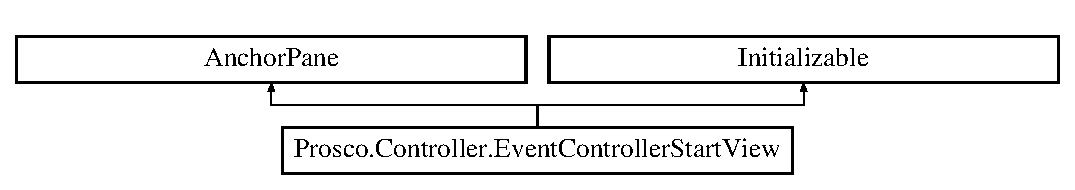
\includegraphics[height=2.000000cm]{class_prosco_1_1_controller_1_1_event_controller_start_view}
\end{center}
\end{figure}
\subsection*{Public Member Functions}
\begin{DoxyCompactItemize}
\item 
\hyperlink{class_prosco_1_1_controller_1_1_event_controller_start_view_a8d3cee31f90605c5516409651f18d3d3}{Event\-Controller\-Start\-View} ()  throws I\-O\-Exception 
\item 
void \hyperlink{class_prosco_1_1_controller_1_1_event_controller_start_view_ae0902afc9a2de5053fa348741ee942ae}{charger\-Vue} ()  throws I\-O\-Exception 
\item 
void \hyperlink{class_prosco_1_1_controller_1_1_event_controller_start_view_aa8abb906535c54da6792eddd453d4296}{get\-Txt\-Recherche\-Ecole} (Action\-Event event)  throws I\-O\-Exception 
\item 
void \hyperlink{class_prosco_1_1_controller_1_1_event_controller_start_view_ac8d58197fce39c723c362f6cbea19d40}{initialize} (U\-R\-L location, Resource\-Bundle resources)
\end{DoxyCompactItemize}
\subsection*{Public Attributes}
\begin{DoxyCompactItemize}
\item 
Auto\-Complete\-Text\-Field$<$ String $>$ \hyperlink{class_prosco_1_1_controller_1_1_event_controller_start_view_a09dbfa302461698bb8489c574860f99f}{Auto\-Complete\-Field}
\end{DoxyCompactItemize}


\subsection{Constructor \& Destructor Documentation}
\hypertarget{class_prosco_1_1_controller_1_1_event_controller_start_view_a8d3cee31f90605c5516409651f18d3d3}{\index{Prosco\-::\-Controller\-::\-Event\-Controller\-Start\-View@{Prosco\-::\-Controller\-::\-Event\-Controller\-Start\-View}!Event\-Controller\-Start\-View@{Event\-Controller\-Start\-View}}
\index{Event\-Controller\-Start\-View@{Event\-Controller\-Start\-View}!Prosco::Controller::EventControllerStartView@{Prosco\-::\-Controller\-::\-Event\-Controller\-Start\-View}}
\subsubsection[{Event\-Controller\-Start\-View}]{\setlength{\rightskip}{0pt plus 5cm}Prosco.\-Controller.\-Event\-Controller\-Start\-View.\-Event\-Controller\-Start\-View (
\begin{DoxyParamCaption}
{}
\end{DoxyParamCaption}
) throws I\-O\-Exception}}\label{class_prosco_1_1_controller_1_1_event_controller_start_view_a8d3cee31f90605c5516409651f18d3d3}


\subsection{Member Function Documentation}
\hypertarget{class_prosco_1_1_controller_1_1_event_controller_start_view_ae0902afc9a2de5053fa348741ee942ae}{\index{Prosco\-::\-Controller\-::\-Event\-Controller\-Start\-View@{Prosco\-::\-Controller\-::\-Event\-Controller\-Start\-View}!charger\-Vue@{charger\-Vue}}
\index{charger\-Vue@{charger\-Vue}!Prosco::Controller::EventControllerStartView@{Prosco\-::\-Controller\-::\-Event\-Controller\-Start\-View}}
\subsubsection[{charger\-Vue}]{\setlength{\rightskip}{0pt plus 5cm}void Prosco.\-Controller.\-Event\-Controller\-Start\-View.\-charger\-Vue (
\begin{DoxyParamCaption}
{}
\end{DoxyParamCaption}
) throws I\-O\-Exception}}\label{class_prosco_1_1_controller_1_1_event_controller_start_view_ae0902afc9a2de5053fa348741ee942ae}
\hypertarget{class_prosco_1_1_controller_1_1_event_controller_start_view_aa8abb906535c54da6792eddd453d4296}{\index{Prosco\-::\-Controller\-::\-Event\-Controller\-Start\-View@{Prosco\-::\-Controller\-::\-Event\-Controller\-Start\-View}!get\-Txt\-Recherche\-Ecole@{get\-Txt\-Recherche\-Ecole}}
\index{get\-Txt\-Recherche\-Ecole@{get\-Txt\-Recherche\-Ecole}!Prosco::Controller::EventControllerStartView@{Prosco\-::\-Controller\-::\-Event\-Controller\-Start\-View}}
\subsubsection[{get\-Txt\-Recherche\-Ecole}]{\setlength{\rightskip}{0pt plus 5cm}void Prosco.\-Controller.\-Event\-Controller\-Start\-View.\-get\-Txt\-Recherche\-Ecole (
\begin{DoxyParamCaption}
\item[{Action\-Event}]{event}
\end{DoxyParamCaption}
) throws I\-O\-Exception}}\label{class_prosco_1_1_controller_1_1_event_controller_start_view_aa8abb906535c54da6792eddd453d4296}
\hypertarget{class_prosco_1_1_controller_1_1_event_controller_start_view_ac8d58197fce39c723c362f6cbea19d40}{\index{Prosco\-::\-Controller\-::\-Event\-Controller\-Start\-View@{Prosco\-::\-Controller\-::\-Event\-Controller\-Start\-View}!initialize@{initialize}}
\index{initialize@{initialize}!Prosco::Controller::EventControllerStartView@{Prosco\-::\-Controller\-::\-Event\-Controller\-Start\-View}}
\subsubsection[{initialize}]{\setlength{\rightskip}{0pt plus 5cm}void Prosco.\-Controller.\-Event\-Controller\-Start\-View.\-initialize (
\begin{DoxyParamCaption}
\item[{U\-R\-L}]{location, }
\item[{Resource\-Bundle}]{resources}
\end{DoxyParamCaption}
)}}\label{class_prosco_1_1_controller_1_1_event_controller_start_view_ac8d58197fce39c723c362f6cbea19d40}


\subsection{Member Data Documentation}
\hypertarget{class_prosco_1_1_controller_1_1_event_controller_start_view_a09dbfa302461698bb8489c574860f99f}{\index{Prosco\-::\-Controller\-::\-Event\-Controller\-Start\-View@{Prosco\-::\-Controller\-::\-Event\-Controller\-Start\-View}!Auto\-Complete\-Field@{Auto\-Complete\-Field}}
\index{Auto\-Complete\-Field@{Auto\-Complete\-Field}!Prosco::Controller::EventControllerStartView@{Prosco\-::\-Controller\-::\-Event\-Controller\-Start\-View}}
\subsubsection[{Auto\-Complete\-Field}]{\setlength{\rightskip}{0pt plus 5cm}Auto\-Complete\-Text\-Field$<$String$>$ Prosco.\-Controller.\-Event\-Controller\-Start\-View.\-Auto\-Complete\-Field}}\label{class_prosco_1_1_controller_1_1_event_controller_start_view_a09dbfa302461698bb8489c574860f99f}


The documentation for this class was generated from the following file\-:\begin{DoxyCompactItemize}
\item 
src/\-Prosco/\-Controller/\hyperlink{_event_controller_start_view_8java}{Event\-Controller\-Start\-View.\-java}\end{DoxyCompactItemize}

\hypertarget{class_prosco_1_1_controller_1_1_event_controller_view_info_ecole}{\section{Prosco.\-Controller.\-Event\-Controller\-View\-Info\-Ecole Class Reference}
\label{class_prosco_1_1_controller_1_1_event_controller_view_info_ecole}\index{Prosco.\-Controller.\-Event\-Controller\-View\-Info\-Ecole@{Prosco.\-Controller.\-Event\-Controller\-View\-Info\-Ecole}}
}
Inheritance diagram for Prosco.\-Controller.\-Event\-Controller\-View\-Info\-Ecole\-:\begin{figure}[H]
\begin{center}
\leavevmode
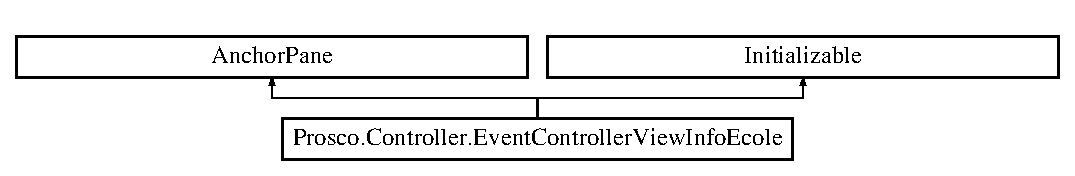
\includegraphics[height=1.911263cm]{class_prosco_1_1_controller_1_1_event_controller_view_info_ecole}
\end{center}
\end{figure}
\subsection*{Public Member Functions}
\begin{DoxyCompactItemize}
\item 
\hyperlink{class_prosco_1_1_controller_1_1_event_controller_view_info_ecole_abf1118ab2040d647c003beaa6d62ba0c}{Event\-Controller\-View\-Info\-Ecole} ()
\item 
void \hyperlink{class_prosco_1_1_controller_1_1_event_controller_view_info_ecole_a4f477e7ec1cad318e6cd6bfc8de750b4}{Back\-Button} (Action\-Event event)  throws I\-O\-Exception 
\item 
void \hyperlink{class_prosco_1_1_controller_1_1_event_controller_view_info_ecole_a31d7b1dcb8a4f2c61d02ed979ae8e31d}{initialize} (U\-R\-L location, Resource\-Bundle resources)
\end{DoxyCompactItemize}
\subsection*{Public Attributes}
\begin{DoxyCompactItemize}
\item 
Text\-Field \hyperlink{class_prosco_1_1_controller_1_1_event_controller_view_info_ecole_a09b2fd3c5664a9eef434358aca15be79}{text\-Field\-Nom\-Ecole}
\item 
Text\-Field \hyperlink{class_prosco_1_1_controller_1_1_event_controller_view_info_ecole_ad6c7a8611ef1f212d8540b3f24982466}{text\-Field\-Num\-Ecole}
\item 
Label \hyperlink{class_prosco_1_1_controller_1_1_event_controller_view_info_ecole_a1710c5a302a88e65a37b6aacc0734ec8}{label\-Nom\-Ecole}
\end{DoxyCompactItemize}


\subsection{Constructor \& Destructor Documentation}
\hypertarget{class_prosco_1_1_controller_1_1_event_controller_view_info_ecole_abf1118ab2040d647c003beaa6d62ba0c}{\index{Prosco\-::\-Controller\-::\-Event\-Controller\-View\-Info\-Ecole@{Prosco\-::\-Controller\-::\-Event\-Controller\-View\-Info\-Ecole}!Event\-Controller\-View\-Info\-Ecole@{Event\-Controller\-View\-Info\-Ecole}}
\index{Event\-Controller\-View\-Info\-Ecole@{Event\-Controller\-View\-Info\-Ecole}!Prosco::Controller::EventControllerViewInfoEcole@{Prosco\-::\-Controller\-::\-Event\-Controller\-View\-Info\-Ecole}}
\subsubsection[{Event\-Controller\-View\-Info\-Ecole}]{\setlength{\rightskip}{0pt plus 5cm}Prosco.\-Controller.\-Event\-Controller\-View\-Info\-Ecole.\-Event\-Controller\-View\-Info\-Ecole (
\begin{DoxyParamCaption}
{}
\end{DoxyParamCaption}
)}}\label{class_prosco_1_1_controller_1_1_event_controller_view_info_ecole_abf1118ab2040d647c003beaa6d62ba0c}


\subsection{Member Function Documentation}
\hypertarget{class_prosco_1_1_controller_1_1_event_controller_view_info_ecole_a4f477e7ec1cad318e6cd6bfc8de750b4}{\index{Prosco\-::\-Controller\-::\-Event\-Controller\-View\-Info\-Ecole@{Prosco\-::\-Controller\-::\-Event\-Controller\-View\-Info\-Ecole}!Back\-Button@{Back\-Button}}
\index{Back\-Button@{Back\-Button}!Prosco::Controller::EventControllerViewInfoEcole@{Prosco\-::\-Controller\-::\-Event\-Controller\-View\-Info\-Ecole}}
\subsubsection[{Back\-Button}]{\setlength{\rightskip}{0pt plus 5cm}void Prosco.\-Controller.\-Event\-Controller\-View\-Info\-Ecole.\-Back\-Button (
\begin{DoxyParamCaption}
\item[{Action\-Event}]{event}
\end{DoxyParamCaption}
) throws I\-O\-Exception}}\label{class_prosco_1_1_controller_1_1_event_controller_view_info_ecole_a4f477e7ec1cad318e6cd6bfc8de750b4}
\hypertarget{class_prosco_1_1_controller_1_1_event_controller_view_info_ecole_a31d7b1dcb8a4f2c61d02ed979ae8e31d}{\index{Prosco\-::\-Controller\-::\-Event\-Controller\-View\-Info\-Ecole@{Prosco\-::\-Controller\-::\-Event\-Controller\-View\-Info\-Ecole}!initialize@{initialize}}
\index{initialize@{initialize}!Prosco::Controller::EventControllerViewInfoEcole@{Prosco\-::\-Controller\-::\-Event\-Controller\-View\-Info\-Ecole}}
\subsubsection[{initialize}]{\setlength{\rightskip}{0pt plus 5cm}void Prosco.\-Controller.\-Event\-Controller\-View\-Info\-Ecole.\-initialize (
\begin{DoxyParamCaption}
\item[{U\-R\-L}]{location, }
\item[{Resource\-Bundle}]{resources}
\end{DoxyParamCaption}
)}}\label{class_prosco_1_1_controller_1_1_event_controller_view_info_ecole_a31d7b1dcb8a4f2c61d02ed979ae8e31d}


\subsection{Member Data Documentation}
\hypertarget{class_prosco_1_1_controller_1_1_event_controller_view_info_ecole_a1710c5a302a88e65a37b6aacc0734ec8}{\index{Prosco\-::\-Controller\-::\-Event\-Controller\-View\-Info\-Ecole@{Prosco\-::\-Controller\-::\-Event\-Controller\-View\-Info\-Ecole}!label\-Nom\-Ecole@{label\-Nom\-Ecole}}
\index{label\-Nom\-Ecole@{label\-Nom\-Ecole}!Prosco::Controller::EventControllerViewInfoEcole@{Prosco\-::\-Controller\-::\-Event\-Controller\-View\-Info\-Ecole}}
\subsubsection[{label\-Nom\-Ecole}]{\setlength{\rightskip}{0pt plus 5cm}Label Prosco.\-Controller.\-Event\-Controller\-View\-Info\-Ecole.\-label\-Nom\-Ecole}}\label{class_prosco_1_1_controller_1_1_event_controller_view_info_ecole_a1710c5a302a88e65a37b6aacc0734ec8}
\hypertarget{class_prosco_1_1_controller_1_1_event_controller_view_info_ecole_a09b2fd3c5664a9eef434358aca15be79}{\index{Prosco\-::\-Controller\-::\-Event\-Controller\-View\-Info\-Ecole@{Prosco\-::\-Controller\-::\-Event\-Controller\-View\-Info\-Ecole}!text\-Field\-Nom\-Ecole@{text\-Field\-Nom\-Ecole}}
\index{text\-Field\-Nom\-Ecole@{text\-Field\-Nom\-Ecole}!Prosco::Controller::EventControllerViewInfoEcole@{Prosco\-::\-Controller\-::\-Event\-Controller\-View\-Info\-Ecole}}
\subsubsection[{text\-Field\-Nom\-Ecole}]{\setlength{\rightskip}{0pt plus 5cm}Text\-Field Prosco.\-Controller.\-Event\-Controller\-View\-Info\-Ecole.\-text\-Field\-Nom\-Ecole}}\label{class_prosco_1_1_controller_1_1_event_controller_view_info_ecole_a09b2fd3c5664a9eef434358aca15be79}
\hypertarget{class_prosco_1_1_controller_1_1_event_controller_view_info_ecole_ad6c7a8611ef1f212d8540b3f24982466}{\index{Prosco\-::\-Controller\-::\-Event\-Controller\-View\-Info\-Ecole@{Prosco\-::\-Controller\-::\-Event\-Controller\-View\-Info\-Ecole}!text\-Field\-Num\-Ecole@{text\-Field\-Num\-Ecole}}
\index{text\-Field\-Num\-Ecole@{text\-Field\-Num\-Ecole}!Prosco::Controller::EventControllerViewInfoEcole@{Prosco\-::\-Controller\-::\-Event\-Controller\-View\-Info\-Ecole}}
\subsubsection[{text\-Field\-Num\-Ecole}]{\setlength{\rightskip}{0pt plus 5cm}Text\-Field Prosco.\-Controller.\-Event\-Controller\-View\-Info\-Ecole.\-text\-Field\-Num\-Ecole}}\label{class_prosco_1_1_controller_1_1_event_controller_view_info_ecole_ad6c7a8611ef1f212d8540b3f24982466}


The documentation for this class was generated from the following file\-:\begin{DoxyCompactItemize}
\item 
src/\-Prosco/\-Controller/\hyperlink{_event_controller_view_info_ecole_8java}{Event\-Controller\-View\-Info\-Ecole.\-java}\end{DoxyCompactItemize}

\hypertarget{class_prosco_1_1_class_1_1_inner_fxml_control}{\section{Prosco.\-Class.\-Inner\-Fxml\-Control Class Reference}
\label{class_prosco_1_1_class_1_1_inner_fxml_control}\index{Prosco.\-Class.\-Inner\-Fxml\-Control@{Prosco.\-Class.\-Inner\-Fxml\-Control}}
}
Inheritance diagram for Prosco.\-Class.\-Inner\-Fxml\-Control\-:\begin{figure}[H]
\begin{center}
\leavevmode
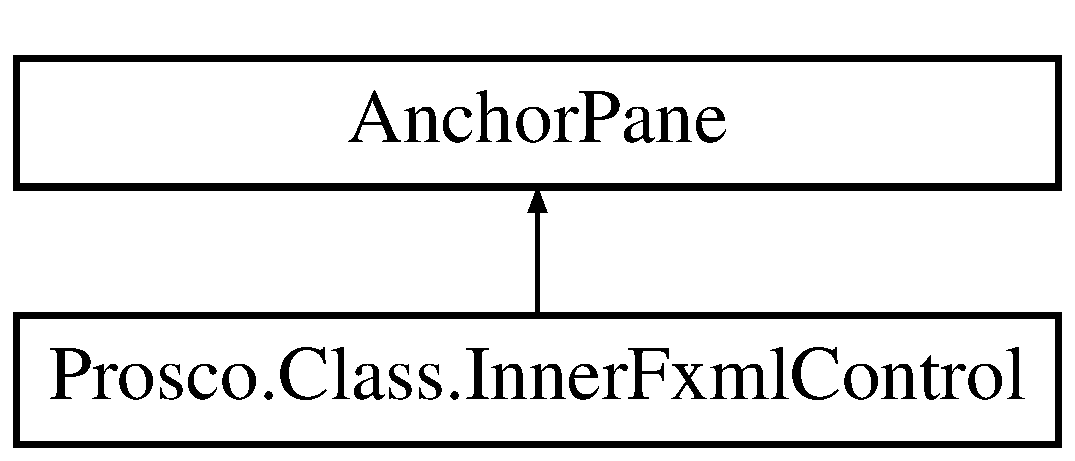
\includegraphics[height=2.000000cm]{class_prosco_1_1_class_1_1_inner_fxml_control}
\end{center}
\end{figure}
\subsection*{Public Member Functions}
\begin{DoxyCompactItemize}
\item 
\hyperlink{class_prosco_1_1_class_1_1_inner_fxml_control_a4e63be96dade1c1b4d5c2d377c8c671d}{Inner\-Fxml\-Control} ()
\end{DoxyCompactItemize}
\subsection*{Public Attributes}
\begin{DoxyCompactItemize}
\item 
Text\-Field \hyperlink{class_prosco_1_1_class_1_1_inner_fxml_control_ac257154f5af4e06ddc41eaa38444a3ab}{text\-Field\-Nom\-Ecole}
\item 
Text\-Field \hyperlink{class_prosco_1_1_class_1_1_inner_fxml_control_ac37709bc3f9f17a4570df610cd7af6d9}{text\-Field\-Num\-Ecole}
\end{DoxyCompactItemize}


\subsection{Constructor \& Destructor Documentation}
\hypertarget{class_prosco_1_1_class_1_1_inner_fxml_control_a4e63be96dade1c1b4d5c2d377c8c671d}{\index{Prosco\-::\-Class\-::\-Inner\-Fxml\-Control@{Prosco\-::\-Class\-::\-Inner\-Fxml\-Control}!Inner\-Fxml\-Control@{Inner\-Fxml\-Control}}
\index{Inner\-Fxml\-Control@{Inner\-Fxml\-Control}!Prosco::Class::InnerFxmlControl@{Prosco\-::\-Class\-::\-Inner\-Fxml\-Control}}
\subsubsection[{Inner\-Fxml\-Control}]{\setlength{\rightskip}{0pt plus 5cm}Prosco.\-Class.\-Inner\-Fxml\-Control.\-Inner\-Fxml\-Control (
\begin{DoxyParamCaption}
{}
\end{DoxyParamCaption}
)}}\label{class_prosco_1_1_class_1_1_inner_fxml_control_a4e63be96dade1c1b4d5c2d377c8c671d}


\subsection{Member Data Documentation}
\hypertarget{class_prosco_1_1_class_1_1_inner_fxml_control_ac257154f5af4e06ddc41eaa38444a3ab}{\index{Prosco\-::\-Class\-::\-Inner\-Fxml\-Control@{Prosco\-::\-Class\-::\-Inner\-Fxml\-Control}!text\-Field\-Nom\-Ecole@{text\-Field\-Nom\-Ecole}}
\index{text\-Field\-Nom\-Ecole@{text\-Field\-Nom\-Ecole}!Prosco::Class::InnerFxmlControl@{Prosco\-::\-Class\-::\-Inner\-Fxml\-Control}}
\subsubsection[{text\-Field\-Nom\-Ecole}]{\setlength{\rightskip}{0pt plus 5cm}Text\-Field Prosco.\-Class.\-Inner\-Fxml\-Control.\-text\-Field\-Nom\-Ecole}}\label{class_prosco_1_1_class_1_1_inner_fxml_control_ac257154f5af4e06ddc41eaa38444a3ab}
\hypertarget{class_prosco_1_1_class_1_1_inner_fxml_control_ac37709bc3f9f17a4570df610cd7af6d9}{\index{Prosco\-::\-Class\-::\-Inner\-Fxml\-Control@{Prosco\-::\-Class\-::\-Inner\-Fxml\-Control}!text\-Field\-Num\-Ecole@{text\-Field\-Num\-Ecole}}
\index{text\-Field\-Num\-Ecole@{text\-Field\-Num\-Ecole}!Prosco::Class::InnerFxmlControl@{Prosco\-::\-Class\-::\-Inner\-Fxml\-Control}}
\subsubsection[{text\-Field\-Num\-Ecole}]{\setlength{\rightskip}{0pt plus 5cm}Text\-Field Prosco.\-Class.\-Inner\-Fxml\-Control.\-text\-Field\-Num\-Ecole}}\label{class_prosco_1_1_class_1_1_inner_fxml_control_ac37709bc3f9f17a4570df610cd7af6d9}


The documentation for this class was generated from the following file\-:\begin{DoxyCompactItemize}
\item 
src/\-Prosco/\-Class/\hyperlink{_inner_fxml_control_8java}{Inner\-Fxml\-Control.\-java}\end{DoxyCompactItemize}

\chapter{File Documentation}
\hypertarget{_app_8java}{\section{src/\-Prosco/\-App/\-App.java File Reference}
\label{_app_8java}\index{src/\-Prosco/\-App/\-App.\-java@{src/\-Prosco/\-App/\-App.\-java}}
}
\subsection*{Classes}
\begin{DoxyCompactItemize}
\item 
class \hyperlink{class_prosco_1_1_app_1_1_app}{Prosco.\-App.\-App}
\end{DoxyCompactItemize}
\subsection*{Packages}
\begin{DoxyCompactItemize}
\item 
package \hyperlink{namespace_prosco_1_1_app}{Prosco.\-App}
\end{DoxyCompactItemize}

\hypertarget{_class_b_d_classes_8java}{\section{src/\-Prosco/\-Class/\-Class\-B\-D\-Classes.java File Reference}
\label{_class_b_d_classes_8java}\index{src/\-Prosco/\-Class/\-Class\-B\-D\-Classes.\-java@{src/\-Prosco/\-Class/\-Class\-B\-D\-Classes.\-java}}
}
\subsection*{Classes}
\begin{DoxyCompactItemize}
\item 
class \hyperlink{class_prosco_1_1_class_1_1_class_b_d_classes}{Prosco.\-Class.\-Class\-B\-D\-Classes}
\end{DoxyCompactItemize}
\subsection*{Packages}
\begin{DoxyCompactItemize}
\item 
package \hyperlink{namespace_prosco_1_1_class}{Prosco.\-Class}
\end{DoxyCompactItemize}

\hypertarget{_class_b_d_ecole_8java}{\section{src/\-Prosco/\-Class/\-Class\-B\-D\-Ecole.java File Reference}
\label{_class_b_d_ecole_8java}\index{src/\-Prosco/\-Class/\-Class\-B\-D\-Ecole.\-java@{src/\-Prosco/\-Class/\-Class\-B\-D\-Ecole.\-java}}
}
\subsection*{Classes}
\begin{DoxyCompactItemize}
\item 
class \hyperlink{class_prosco_1_1_class_1_1_class_b_d_ecole}{Prosco.\-Class.\-Class\-B\-D\-Ecole}
\end{DoxyCompactItemize}
\subsection*{Packages}
\begin{DoxyCompactItemize}
\item 
package \hyperlink{namespace_prosco_1_1_class}{Prosco.\-Class}
\end{DoxyCompactItemize}

\hypertarget{_connect_b_d_8java}{\section{src/\-Prosco/\-Class/\-Connect\-B\-D.java File Reference}
\label{_connect_b_d_8java}\index{src/\-Prosco/\-Class/\-Connect\-B\-D.\-java@{src/\-Prosco/\-Class/\-Connect\-B\-D.\-java}}
}


Classe qui permet de cr�er la connexion aux bases de donn�es  


\subsection*{Classes}
\begin{DoxyCompactItemize}
\item 
class \hyperlink{class_prosco_1_1_class_1_1_connect_b_d}{Prosco.\-Class.\-Connect\-B\-D}
\end{DoxyCompactItemize}
\subsection*{Packages}
\begin{DoxyCompactItemize}
\item 
package \hyperlink{namespace_prosco_1_1_class}{Prosco.\-Class}
\end{DoxyCompactItemize}


\subsection{Detailed Description}
Classe qui permet de cr�er la connexion aux bases de donn�es \begin{DoxyAuthor}{Author}
bfaliu 
\end{DoxyAuthor}
\begin{DoxyVersion}{Version}
1.\-0 
\end{DoxyVersion}
\begin{DoxyDate}{Date}
29/09/2013 
\end{DoxyDate}

\hypertarget{_inner_fxml_control_8java}{\section{src/\-Prosco/\-Class/\-Inner\-Fxml\-Control.java File Reference}
\label{_inner_fxml_control_8java}\index{src/\-Prosco/\-Class/\-Inner\-Fxml\-Control.\-java@{src/\-Prosco/\-Class/\-Inner\-Fxml\-Control.\-java}}
}
\subsection*{Classes}
\begin{DoxyCompactItemize}
\item 
class \hyperlink{class_prosco_1_1_class_1_1_inner_fxml_control}{Prosco.\-Class.\-Inner\-Fxml\-Control}
\end{DoxyCompactItemize}
\subsection*{Packages}
\begin{DoxyCompactItemize}
\item 
package \hyperlink{namespace_prosco_1_1_class}{Prosco.\-Class}
\end{DoxyCompactItemize}

\hypertarget{_event_controller_start_view_8java}{\section{src/\-Prosco/\-Controller/\-Event\-Controller\-Start\-View.java File Reference}
\label{_event_controller_start_view_8java}\index{src/\-Prosco/\-Controller/\-Event\-Controller\-Start\-View.\-java@{src/\-Prosco/\-Controller/\-Event\-Controller\-Start\-View.\-java}}
}
\subsection*{Classes}
\begin{DoxyCompactItemize}
\item 
class \hyperlink{class_prosco_1_1_controller_1_1_event_controller_start_view}{Prosco.\-Controller.\-Event\-Controller\-Start\-View}
\end{DoxyCompactItemize}
\subsection*{Packages}
\begin{DoxyCompactItemize}
\item 
package \hyperlink{namespace_prosco_1_1_controller}{Prosco.\-Controller}
\end{DoxyCompactItemize}

\hypertarget{_event_controller_view_info_ecole_8java}{\section{src/\-Prosco/\-Controller/\-Event\-Controller\-View\-Info\-Ecole.java File Reference}
\label{_event_controller_view_info_ecole_8java}\index{src/\-Prosco/\-Controller/\-Event\-Controller\-View\-Info\-Ecole.\-java@{src/\-Prosco/\-Controller/\-Event\-Controller\-View\-Info\-Ecole.\-java}}
}
\subsection*{Classes}
\begin{DoxyCompactItemize}
\item 
class \hyperlink{class_prosco_1_1_controller_1_1_event_controller_view_info_ecole}{Prosco.\-Controller.\-Event\-Controller\-View\-Info\-Ecole}
\end{DoxyCompactItemize}
\subsection*{Packages}
\begin{DoxyCompactItemize}
\item 
package \hyperlink{namespace_prosco_1_1_controller}{Prosco.\-Controller}
\end{DoxyCompactItemize}

%--- End generated contents ---

% Index
\newpage
\phantomsection
\addcontentsline{toc}{part}{Index}
\printindex

\end{document}
